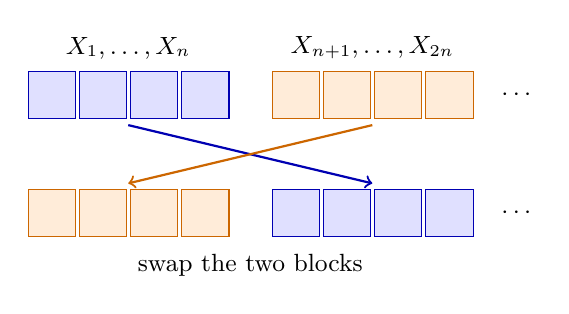
\begin{tikzpicture}[x=1cm,y=1cm]
\foreach \i in {0,1,2,3} {
  \draw[fill=blue!12,draw=blue!70!black] (\i*0.65,1.5) rectangle ++(0.6,0.6);
  \draw[fill=orange!15,draw=orange!80!black] (3.1+\i*0.65,1.5) rectangle ++(0.6,0.6);
  \draw[fill=orange!15,draw=orange!80!black] (\i*0.65,0) rectangle ++(0.6,0.6);
  \draw[fill=blue!12,draw=blue!70!black] (3.1+\i*0.65,0) rectangle ++(0.6,0.6);
}
\node[font=\small] at (1.27,2.4) {$X_1,\ldots,X_n$};
\node[font=\small] at (4.37,2.4) {$X_{n+1},\ldots,X_{2n}$};
\node[font=\small] at (6.2,1.8) {$\cdots$};
\node[font=\small] at (6.2,0.3) {$\cdots$};
\draw[->,blue!70!black,thick] (1.27,1.42)--(4.37,0.68);
\draw[->,orange!80!black,thick] (4.37,1.42)--(1.27,0.68);
\node[font=\small] at (2.82,-0.36) {swap the two blocks};
\end{tikzpicture}
